%!TEX root = farm.tex

\section{Compiler and Debugging Environment}\label{sec:design}

This section describes the design and implementation of our compiler and
debugging environment for NVIDIA's GPU microcontrollers.

\subsection{GPU microcontroller}

\begin{table}[tb]
\caption{Microcontroller Specifications in GF100 } 
\label{tab:fermi}
% $B:81&$N7S@~$O$D$1$:!$0lHV>e$N7S@~$OFs=E@~(B
\hbox to\hsize{\hfil
\begin{tabular}{|l|r|r|}\hline
Name 		&	HUB	   & GPC\\\hline
Architecture &	Fermi   & Fermi \\\hline
Number		& 1 & 4\\\hline
Bit 		&	32bit  & 32bit\\\hline
Code size  &	16,384 byte  & 8,192 byte\\\hline
Data size  &	4,096 byte  & 2,048 byte\\\hline
% \multicolumn{4}{l}{type-1\,: enumerate$BEy(B\quad type-2\,: enumerate*$BEy(B}\\
% \multicolumn{4}{l}{type-3\,: Enumerate$BEy(B\quad type-4\,: ENUMERATE$BEy(B}\\
\end{tabular}\hfil}
\end{table}

This research use the microcontroller of Nvidia's Fermi architecture such as GF100 (GeForce GTX480).
In GF100, a Streaming Multiprocessor (SM) consists of 32 CUDA cores, and a Graphical Processor Cluster (GPC) consists of 4 SM's, and GF100 consist of 4 GPC's. Thus GF100 mounted 512 CUDA cores. Since one full SM is disabled. GF100 has 480 valid CUDA cores.
Since maximum code size of the microcontroller is limited to 16KB as indicated in Table \ref{tab:fermi}, developers should carefully design the firmware.

\subsection{The compiler for GPU microcontroller}
The compiler for GPU microcontroller generates object code of GPU microcontroller manufactured by NVIDIA.
\subsubsection{The overall flow}\label{section:flow}
\begin{figure*}
\begin{center}
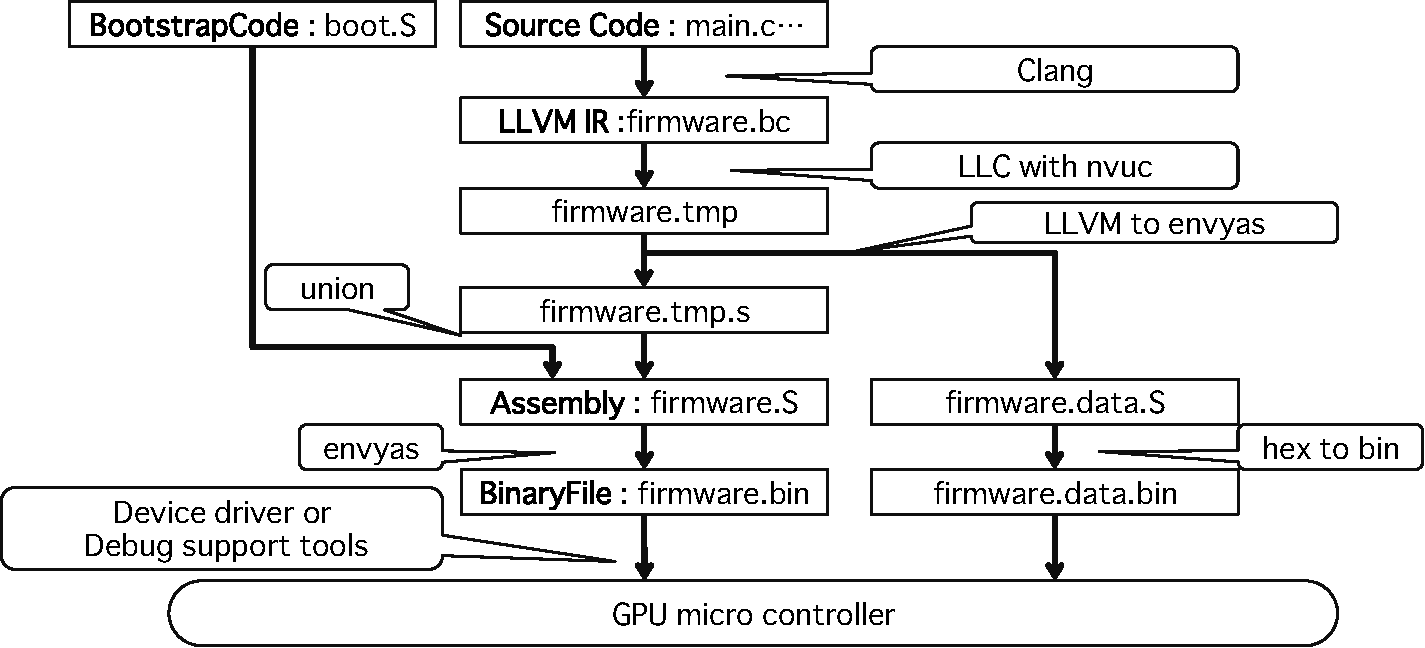
\includegraphics[width=12cm]{./img/step_compiler.pdf}
\end{center}
\caption{Detail of Compiler for GPU Microcontroller}
\label{fig:compiler}
\end{figure*}


The compiler for GPU microcontroller implemented using the LLVM.
Figure \ref{fig:compiler} shows an overall view of the compiler for GPU microcontroller.
The main flow of the compilation is Clang done generate LLVM IR from the source of the C language in the first,
Next then, LLC generates assembly code from LLVM IR.
After, assembly code divided to code part and data part, code part unions bootstrap code.

Finally, envyas generates an executable file.
The executable file can be run using the debugging support tool or device driver.
If developer develops the firmware in this development environment that only need to write the code for the C language.

\begin{description}
\item[ (1) Clang]\mbox{}\\
Clang is a frontend that generates IR for LLVM from C language source codes.

\begin{figure}
\begin{center}
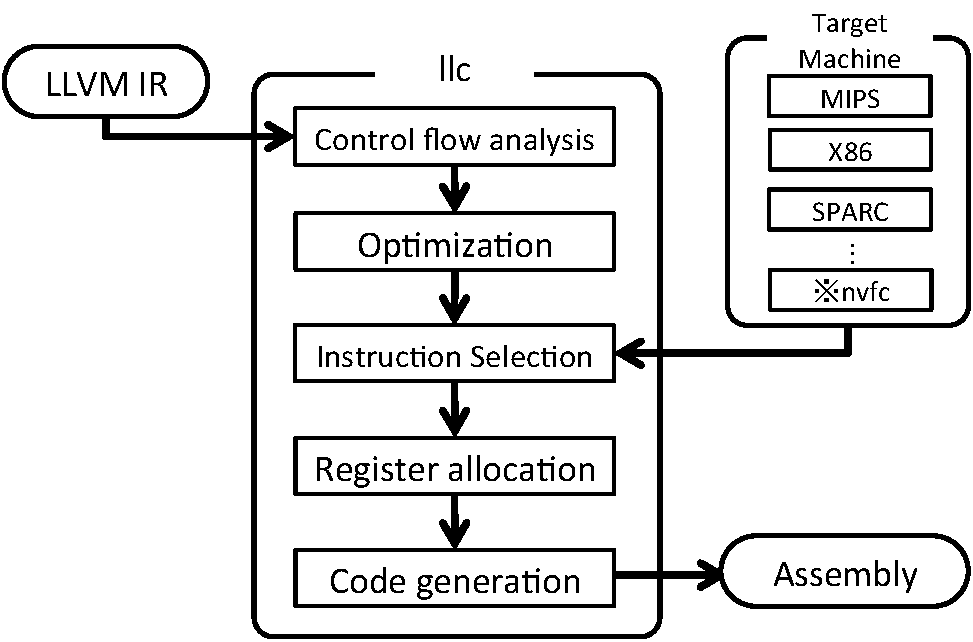
\includegraphics[width=6cm]{./img/llc.pdf}
\end{center}
\caption{Step of code generation in LLC}
\label{fig:llc}
\end{figure}

\begin{figure*}
\begin{center}
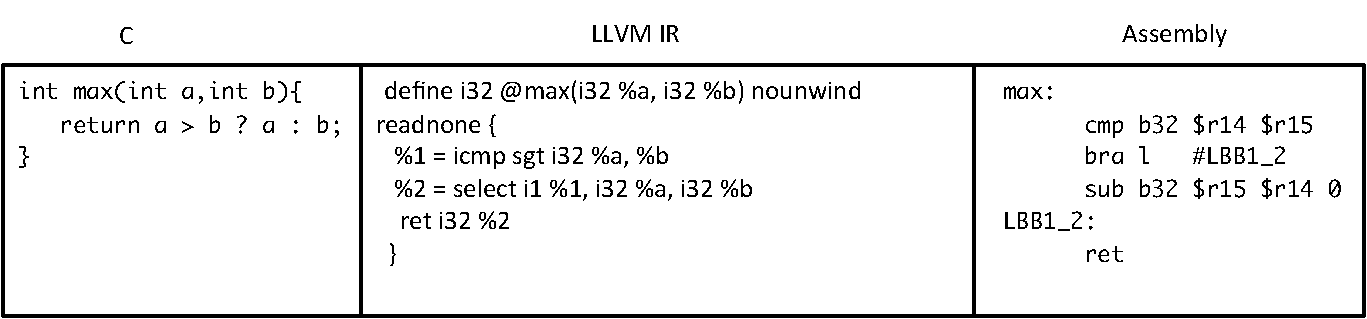
\includegraphics[width=12cm]{./img/llvm_code.pdf}
\end{center}
\caption{C source code and generated code. Left : C, Center : LLVM IR, Right : Assembly}
\label{fig:llvm_code}
\end{figure*}
\item[ (2) LLC with nvfuc]\mbox{}\\
As mentioned Section \ref{set:backend}, LLC is the backend of LLVM that compiles LLVM IR code into assembly language for a specified architecture.
Figure \ref{fig:llc} shows LLC flow.
There are five steps to convert an LLVM IR to specific assembly code; flow analysis, optimization, instruction selection, register allocation, code generation.
The flow is not depend on the target machine agnostic has been standardized.
LLC reads the configuration of the target machine at the time of the instruction selection and selects the instruction and register to meet the specifications of each machine. 
A new configuration called nvfc (NVidia Firmware Compiler) for GPU microcontroller manufactured by NVIDIA is added to target machine configurations.

\item[ (3) LLVM to envyas]\mbox{}\\
``LLVM to envyas'' divides the generated assembly code into code section and data section.
``LLVM to envyas'' combines code section and BootstrapCode including code to set up an interrupt handler and a call main function.
Further ``LLVM to envyas'' replaces labels of code section to data address.
\item[ (4) envyas]\mbox{}\\
As mentioned in Section \ref{sec:design},
``envyas'' is assembler for the GPU micro controller and is included in the envytools.
The envyas generates the execution files from generated the code section by Step (3).

\item[ (5) hex to bin]\mbox{}\\
``hex to bin'' converts to the data portion split Step (3) to an executable file.

\item[ (6) Running the firmware]\mbox{}\\
There are two ways to run the firmware: incorporating the firmware into the device driver, or using the debugging support tool.
The device driver and the debugging support tool load the binary file of the firmware at boot time.
\end{description}

\subsubsection{The generated code}
Figure \ref{fig:llvm_code} shows example of C language source codes, LLVM IR code, and assembly code.
Left is C language source codes, center is LLVM IR code that is generated by \ref{section:flow}(1), right is assembly code that is generated by \ref{section:flow}(3).

\begin{figure}
\begin{center}
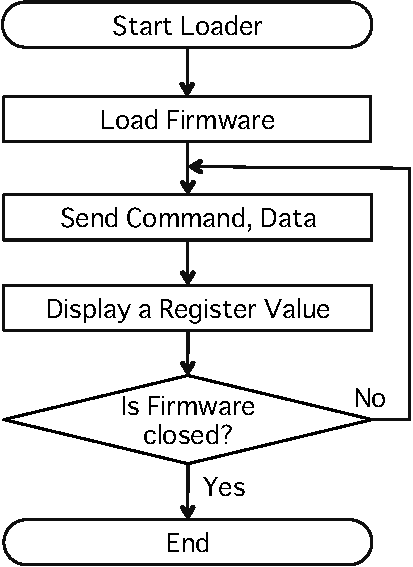
\includegraphics[width=3cm]{./img/loader.pdf}
\end{center}
\caption{Flowchart of Debugging Support Tool}
\label{fig:loader}
\end{figure}

\begin{figure*}
\begin{center}
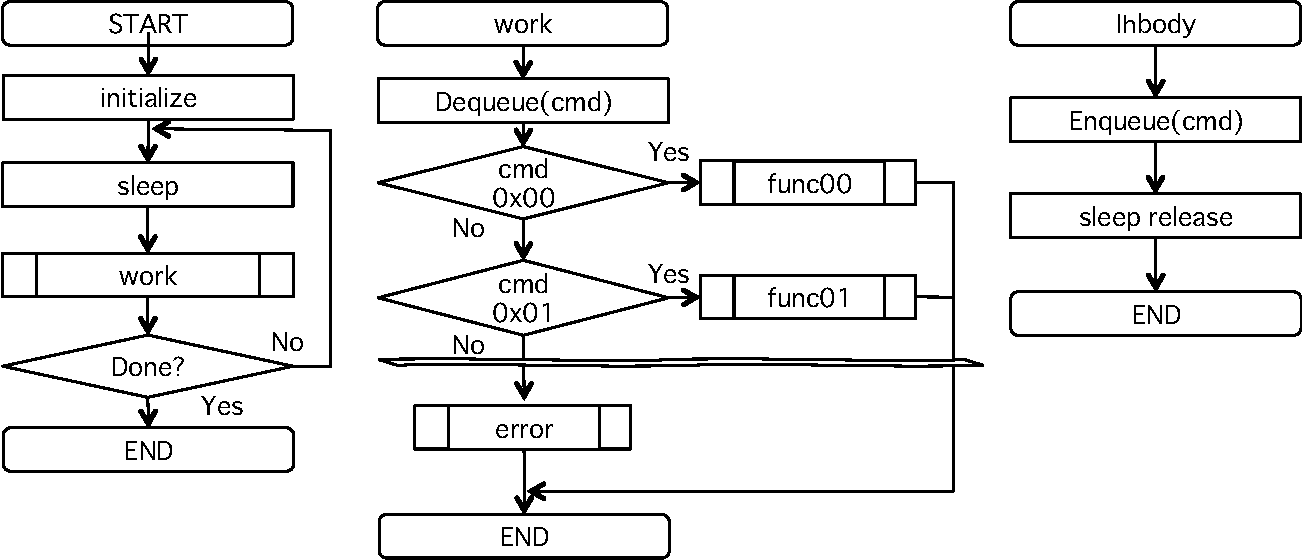
\includegraphics[width=12cm]{./img/firmware.pdf}
\end{center}
\caption{Flowchart of Our Firmware }
\label{fig:firmware}
\end{figure*}


\subsection{Debugging support tool}
Debugging support tool is to load the firmware, to send commands and data, and to display a register value of GPU.
Figure \ref{fig:loader} shows the flow of this tool flow, we describe use it.
Microcontrollers memory space map to  CPU memory space in MMIO (Memory Mapped IO).

\begin{description}
\item[ (1) Load the firmware]\mbox{}\\
Debugging support tool load the HUB firmware and GPC firmware executable code to mapping address by MMIO. 
After the load completion, this firmware runs by set a flag in the specified register.
\item[ (2) Sends commands and data]\mbox{}\\
A processing on microcontroller is suspended until receives a command.
The debugging support tool sends the command.
After an interrupt is executed by the command, the processing is resumed,

\item[ (3) Display a register] \mbox{}\\
The microcontroller has the register may be used freely on the host side.
The register is used for execute completion flag by the traditional firmware.
Thus we assumed that the register is used for the same purpose during debugging time, 
the register value is displayed.
\end{description}


\subsection{Firmware development}
In this section, we describe the our developing firmware on HUB.
Figure \ref{fig:firmware} shows that firmware flow chart.
The Firmware is started by setting the value in the register.

\begin{description}
\item[ (1) initialize]\mbox{}\\
The firmware sets the interrupt handler and get the data when started.
Next then Step(2).
\item[ (2) sleep]\mbox{}\\
The firmware makes the shift to the standby state, which wait for the receive command by the device driver or the debug support tools.
The firmware interrupt occurs when the firmware received command, which started ``ihbody''. 

\item[ (3) ihbody] \mbox{}\\
``ihbody'' enqueued command, and then it releases wait state of firmware.
\item[ (4) work] \mbox{}\\
``work'' function is called when the wait state of firmware is released.
``work'' calls the function after the dequeue.
It will check the end flag of firmware after the function execution.
\end{description}
We can recognize from what has been said that the firmware controlled by execute the function is better suited command.

